\documentclass[conference]{IEEEtran}
\IEEEoverridecommandlockouts
% The preceding line is only needed to identify funding in the first footnote. If that is unneeded, please comment it out.
\usepackage{cite}
\usepackage{amsmath,amssymb,amsfonts}
\usepackage{algorithmic}
\usepackage{graphicx}
\usepackage{textcomp}
\usepackage{subcaption}
\usepackage{multicol}
\usepackage{xcolor}
\def\BibTeX{{\rm B\kern-.05em{\sc i\kern-.025em b}\kern-.08em
    T\kern-.1667em\lower.7ex\hbox{E}\kern-.125emX}}
\begin{document}

\title{P-BOT: Your personal PDF chatbot\\
{\footnotesize \textsuperscript{*}Note: Sub-titles are not captured in Xplore and
should not be used}
\thanks{Identify applicable funding agency here. If none, delete this.}
}

\author{\IEEEauthorblockN{1\textsuperscript{st} Abhijit Patil}
\IEEEauthorblockA{\textit{dept. name of organization (of Aff.)} \\
\textit{name of organization (of Aff.)}\\
City, Country \\
email address or ORCID}
\and
\IEEEauthorblockN{2\textsuperscript{nd} Shubhi Parashar}
\IEEEauthorblockA{\textit{dept. name of organization (of Aff.)} \\
\textit{name of organization (of Aff.)}\\
City, Country \\
email address or ORCID}
\and
\IEEEauthorblockN{3\textsuperscript{rd} Parth Shah}
\IEEEauthorblockA{\textit{dept. name of organization (of Aff.)} \\
\textit{name of organization (of Aff.)}\\
City, Country \\
email address or ORCID}
\and
\IEEEauthorblockN{4\textsuperscript{th} Manan Salia}
\IEEEauthorblockA{\textit{dept. name of organization (of Aff.)} \\
\textit{name of organization (of Aff.)}\\
City, Country \\
email address or ORCID}
}

\maketitle

\begin{abstract}
In an era where PDFs store vast amounts of information, the laborious task of manually sifting through extensive, complex documents hinders academic research and knowledge management. P-BOT, the Personalized PDF Chat Bot, emerges as an ingenious solution. Leveraging advanced NLP and ML techniques, P-BOT parses PDFs, creating structured knowledge bases for each. It offers a user-friendly chat interface, allowing plain language queries to extract concise, accurate answers directly from the PDF content. P-BOT revolutionizes PDF interaction, bridging the gap between information and accessibility, ultimately enhancing academic research and knowledge utilization through its innovative fusion of NLP and ML technologies.
\end{abstract}
\parskip=0.5\baselineskip
\begin{IEEEkeywords}
Chatbot, PDF, GPT, LLM, Infromation Retrieval, P-BOT.
\end{IEEEkeywords}

\section{Introduction}

In response to the challenges posed by digital intelligence in the digital economy, the emergence of Artificial Intelligence Generated Content (AIGC)[1-3] has been noteworthy. AIGC leverages artificial intelligence to facilitate or even replace manual content generation, generating content in accordance with user-provided keywords or specifications. The continuous advancement of large-scale model algorithms has significantly enhanced the capabilities of AIGC, rendering it a promising generative tool that enhances convenience in various aspects of our lives. Positioned as an upstream technology, AIGC possesses limitless potential to support diverse downstream applications. A pivotal transformation is underway in the realm of content creation and knowledge representation due to the widespread adoption of large artificial intelligence models such as ChatGPT[2]. AIGC, driven by these generative large AI algorithms, is at the forefront of this paradigm shift. It empowers users by aiding or even substituting human efforts in generating extensive, top-tier, and remarkably human-like content swiftly and cost-effectively, all hinging on user-provided prompts. 

\parskip=0.5\baselineskip

Generative AI[4] stands as a pivotal component within the Artificial Intelligence Generated Content (AIGC) consortium, playing a significant role in shaping the future of AI-driven interactions. Generative AI facilitates the development of conversational agents and chatbots capable of engaging in dynamic and contextually relevant interactions, thereby enhancing user experiences across a wide range of applications, from customer service to content generation. This innovative technology continues to evolve, pushing the boundaries of what AI can achieve in understanding and generating human language, ultimately paving the way for more intelligent and responsive AI systems.

Leveraging Generative AI represents a strategic advantage, as it enables the integration of advanced tools capable of addressing inquiries pertaining to PDF documents. In the contemporary digital era, libraries have evolved beyond their traditional physical confines to encompass a vast array of online resources tailored to serve their patrons. A widely adopted format for these digital resources is the Portable Document Format (PDF), which facilitates the seamless dissemination of information while preserving the original document's layout and formatting. Consequently, PDFs have gained popularity, particularly for the storage and distribution of academic articles and research reports. Nevertheless, PDFs present a unique challenge within library systems, primarily stemming from their limited interactivity when compared to dynamic web pages and other digital content sources. Unlike more interactive resources, PDFs lack essential features that enable users to conduct in-document searches, annotate text, or navigate through different sections seamlessly. This deficiency can result in user frustration and disengagement, particularly when users seek more interactive functionalities. Consequently, addressing the issue of PDF interaction within library systems emerges as a pivotal endeavor. The enhancement of user engagement and satisfaction relies on the provision of more interactive PDF experiences. Libraries can significantly elevate the user experience by offering interactive PDFs, thereby fostering a greater likelihood of users returning to the library as a valuable and user-centric resource.

A promising solution to the aforementioned challenge is the introduction of the P-BOT, an acronym denoting the "Personalized PDF Chat-BOT." The P-BOT represents an innovative online software platform that leverages the formidable capabilities of the ChatGPT API, offering users a more intuitive and seamless method for engaging with PDF documents. Through seamless integration of the P-BOT into library systems, patrons gain access to a chat-based interface that enables efficient and natural interactions with digital resources, including books, research papers, theses, manuals, essays, and a diverse range of academic content. P-BOT empowers users to pose queries, request assistance, and effortlessly navigate through PDF documents, thus serving as a valuable and transformative addition to library systems. This cutting-edge tool not only enhances user experiences but also streamlines the accessibility and usability of library resources, aligning perfectly with the evolving needs of modern library patrons, researchers, and scholars, thereby contributing to the advancement of knowledge dissemination. P-BOT will incorporate the feature of uploading multiple PDFs, including PDFs of substantial length, such as those spanning up to 1,000 pages.






\section{Literature Survey}

\subsection{History of Text Extraction}

In the late 1990s, as the usage of PDF documents surged, initial efforts were made to extract text from these files. These early text extraction techniques primarily focused on dissecting the PDF structure to identify and retrieve text content. However, they encountered limitations, particularly in terms of accuracy and their ability to preserve document formatting. 

To address these challenges, Optical Character Recognition (OCR) technology was introduced, aiming to convert printed and handwritten text into digital format. OCR's primary objective was to facilitate the transition from paper-based content to the digital realm, enhancing accessibility, editability, and searchability. It not only automated data entry, reducing errors and costs, but also streamlined information retrieval from scanned documents and archives. OCR played a pivotal role in extracting text from tangible documents, images, and PDFs, making content searchable, editable, and available for diverse applications. Moreover, it significantly improved text accessibility for individuals with visual impairments by converting text into a readable format for assistive technologies. The introduction of OCR marked a groundbreaking transformation in how text-based information is managed, bridging the analog and digital realms.

Tesseract OCR, an open-source Optical Character Recognition engine developed by Google, is renowned for its exceptional precision in identifying printed text within scanned documents, images, and PDFs. Tesseract is compatible with various languages, capable of extracting text from diverse fonts and text sizes. Its adaptability and ongoing enhancements have solidified its status as a favored solution for automating data entry, digitizing printed resources, enabling text searches within images, and supporting a variety of applications that require the transformation of visual text into machine-readable text.

While traditional OCR technology excelled within predefined formats and fonts, machine learning (ML) and deep learning have emerged as superior alternatives due to their adaptability, superior accuracy, and contextual comprehension of text. These models surpass the rigid constraints of OCR, accommodating a wide range of document layouts, languages, and even handwritten content. Their versatility enables the precise extraction of text, making them suitable for handling complex documents. Moreover, these models continuously improve their performance through fine-tuning with new data, ensuring their ongoing relevance and effectiveness in an ever-evolving digital landscape.

The utilization of machine learning and deep learning methods, including natural language processing (NLP) models, has led to significant advancements in text extraction from PDFs. These advanced models excel at identifying and extracting text content from intricate PDF documents, including those with multiple columns, tables, and a wide variety of fonts, further enhancing the efficiency and accuracy of text extraction processes.

\subsection{History of Text Generation}

Understanding the landscape of generative AI models is crucial for making informed choices regarding their suitability for various applications within our software platform. The foundations of generative models trace back to the 1950s when pioneering efforts led to the development of Hidden Markov Models (HMMs)[5,6] and Gaussian Mixture Models (GMMs)[7]. These early models exhibited the capability to generate sequential data, a milestone achievement with notable applications in speech recognition and time series analysis. However, it was not until the advent of deep learning in more recent years that generative models truly began to shine. Deep learning models, including neural networks, Recurrent Neural Networks (RNNs), and Convolutional Neural Networks (CNNs), have played a pivotal role in significantly enhancing the performance and versatility of generative AI. Their ability to learn complex patterns, capture long-term dependencies, and generate high-dimensional data has revolutionized the field.

\subsubsection{Language Models}

Statistical language models play a fundamental role in natural language processing by estimating the probability distribution of natural language. These models are dedicated to estimating the probability of generating a given sentence or predicting the content of the next part of a sentence, which is essential for various downstream NLP tasks. Various modeling methods have been developed to address this, reflecting the technical advancements in the field. Early n-gram language models rely on frequency statistics of n-grams, but they have limitations in handling larger context and symbol combinations. Neural language models (NLM) introduced more complex structures, such as multilayer perceptrons, convolutional neural networks, and recurrent neural networks, improving the representation of words and their context-aware dynamic nature through low-dimensional embeddings.

Since 2018, pre-trained language models (PLM) have gained attention, particularly those based on self-supervised learning over large-scale text data. Notable models like ELMo, BERT, and GPT-3 have demonstrated remarkable performance in various NLP tasks. PLMs offer dynamic context-aware representations and serve as a unified framework for NLP tasks. They have three typical model structures: autoregressive LM, autoencoding LM, and hybrid LM, represented by GPT, BERT, and T5, respectively. Autoregressive LM focuses on token-by-token word prediction, while autoencoding LM masks words in sentences, employs bidirectional encoding, and predicts the masked words based on context. Hybrid LM combines these approaches. BERT's success has led to its widespread adoption in academia and industry due to its strong performance in NLP tasks.

Leveraging the Transformer architecture, OpenAI has developed a series of GPT models, including GPT-1, GPT-2, GPT-3, and GPT-4. These models have demonstrated improvements in language understanding and generation, with GPT-3 being particularly noteworthy for its excellence in text generation tasks and support for zero-shot and few-shot learning scenarios. OpenAI has further advanced large-scale language models with models like GPT-3.5 series, which includes Code-davinci and Text-davinci models. These models have enabled users to leverage advanced language capabilities through APIs and playgrounds. GPT-4, the latest milestone, is a large multimodal model, showing enhanced capabilities in understanding nuanced instructions.

The development of artificial intelligence has highlighted the power of large models in learning complex features and patterns from raw data, ultimately leading to stronger data understanding and generation capabilities. These large-scale pre-trained language models exhibit better generalization and general task processing capabilities. The autoregressive language modeling approach adopted by GPT-3 and its successors has proven advantageous in directly utilizing natural language to describe various tasks in different domains. Researchers are now eager to explore the transparency and capabilities of GPT-4 in further advancing the field of artificial intelligence. These advancements signify the critical role that language models play in modern NLP and AI technologies.

Among the earliest methods for sentence generation, N-gram language modeling[8-10] stands as a foundational approach in the realm of Natural Language Processing (NLP). N-grams represent contiguous sequences of words, symbols, or tokens in textual or speech data, defined as neighboring sequences within a given document. These N-grams are integral to a wide array of applications in NLP, extending their influence to domains such as statistical natural language processing, speech recognition, phonemes, machine translation, predictive text input, and more, where the modeling inputs rely on N-gram distributions. N-grams themselves manifest as co-occurring words or items within a specific window, advanced by a fixed number of words or tokens, often referred to as "k." These co-occurring words are termed "n-grams," with "n" signifying the length of the word string considered in constructing these n-grams. The spectrum encompasses unigrams (single words), bigrams (two-word sequences), trigrams (three-word sequences), 4-grams, 5-grams, and so forth. N-grams are harnessed extensively in NLP, text mining, and various natural language processing tasks. Language model development in NLP, for instance, leverages not just unigram models but extends to bigram and trigram models. Major tech companies, including Google and Microsoft, have ventured into constructing expansive web-scale n-gram models, which find utility in NLP tasks like spelling correction, word segmentation, and text summarization. Furthermore, N-grams are vital in crafting features for supervised Machine Learning models, such as Support Vector Machines (SVMs), Maximum Entropy (MaxEnt) models, and Naive Bayes classifiers. The fundamental concept lies in enriching the feature space with tokens like bigrams, trigrams, and more advanced n-grams, transcending the limitations of relying solely on unigrams.


\begin{figure*}
    \centering
    \includegraphics[width=\textwidth]{LM_TYPES}
    \caption{There three typical types of PLM: autoregressive LM, autoencoder LM and hybrid LM. Their working mechanisms are listed and compared in this
table taken from Tianyu Wu et al. [A Brief Overview of ChatGPT: The History, Status Quo and Potential Future Development]}
    \label{fig:your_image_label}
\end{figure*}


The utilization of N-gram language modeling has indeed played a pivotal role in advancing the domain of text generation. However, it is essential to recognize that its effectiveness encounters constraints, particularly when dealing with longer and more intricate sentences. These limitations have acted as a catalyst for the emergence of recurrent neural networks (RNNs), which represent a groundbreaking development in the realm of language modeling tasks. In their initial iterations, RNNs brought forth a crucial innovation by granting the ability to model longer dependencies within textual data. This innovation opened doors to the generation of more extensive and intricate sentences, marking a significant leap in the quest for improved text generation techniques.



In the broader context of natural language processing (NLP), it's important to note that the narrative of innovation did not begin with RNNs alone. Convolutional Neural Networks (CNNs) had already made substantial contributions to the field before the advent of RNNs. These two deep neural network (DNN) architectures, CNNs and RNNs, have become foundational tools in NLP tasks. CNNs, in particular, excel in capturing position-invariant features, making them adept at identifying local patterns, n-grams, and various features within textual data. Their versatility has been evident across an array of NLP tasks, encompassing text classification, semantic similarity analysis, named entity recognition, document classification, question answering, and text generation. Nonetheless, it's essential to acknowledge that while CNNs offer compelling advantages, they may not be universally suitable for all NLP applications. This consideration arises from the inherent design of CNNs, which is not primarily tailored for sequential data processing. In the domain of NLP, textual data inherently comprises sequences of words or tokens, presenting a unique challenge when employing CNNs for efficient data processing.


On the contrary, RNNs are a specialized class of neural networks explicitly engineered to handle sequential data. In a standard Recurrent Neural Network, each output depends on both the current input and the internal memory or hidden state inherited from the previous step. This intrinsic mechanism empowers RNNs to retain vital information about past inputs, enabling them to effectively capture intricate sequential relationships in data. 




Introduced in 1997, Long Short-Term Memory networks, or LSTMs, represent a pivotal advancement in the realm of recurrent neural networks (RNNs). LSTMs were specifically designed to tackle the daunting challenge of the vanishing gradient problem that often plagues the training of deep neural networks, particularly in the context of RNNs and certain deep feedforward networks. The vanishing gradient problem emerges when the gradients of the loss function with respect to the network's parameters dwindle to nearly zero as they propagate backward through the network's layers during the training process.


LSTMs excel in capturing long-term dependencies within sequences, offering a solution to issues related to backflow errors and the need to minimize time intervals. Unlike earlier methods, LSTMs swiftly learn to discern multiple occurrences of a specific element in an input sequence, even when those occurrences are widely spaced, without relying on specific short-time-lag training examples. These networks demonstrate the remarkable ability to effectively capture and connect information across substantial time intervals, surpassing 1000 discrete-time steps. This capability is achieved by maintaining a consistent flow of error information through dedicated units referred to as "constant error carousels." Additionally, LSTMs employ multiplicative gate units that learn to regulate access to this constant error flow, determining when to open or close it.

However, it's crucial to acknowledge that LSTMs are not without their challenges. They are notably challenging to train due to their involvement in very long gradient paths. LSTMs are susceptible to overfitting, especially when dealing with limited datasets. Effective performance often necessitates a substantial amount of training data, and they may struggle to generalize effectively when data is scarce. Furthermore, LSTMs can be memory-intensive, particularly when dealing with extended sequences or complex model architectures. Another notable aspect is that LSTMs are frequently regarded as inscrutable models, which can pose challenges in understanding the decision-making processes underlying their predictions. This opacity becomes a significant concern in contexts where transparency and interpretability hold paramount importance.



In the pursuit of generating sentences with similar attributes using Long Short-Term Memory networks (LSTMs), an innovative approach, the Syntactic and Semantic LSTM (SSLSTM), was introduced. The SSLSTM approach, as detailed in "Generating and Measuring Similar Sentences Using Long Short-Term Memory and Generative Adversarial Networks," leverages both syntactic and semantic information inherent in sentences to gauge their similarity. At the heart of SSLSTM lies its sentence model, a critical component that harnesses sentence-syntactic and word-semantic features to effectively encapsulate the fundamental linguistic characteristics of input sentences.


The process begins with the segmentation of text into individual words, employing word embeddings to encode these words with contextual information. CoreNLP, a natural language processing toolkit, is subsequently employed to generate related sentences by extracting syntactic word relationships, thereby adding a layer of syntactic understanding to the similarity measurement. Additionally, an offline package of WordNet 3 comes into play, serving the purpose of identifying analogous nouns within sentences and simplifying their overall complexity. This multi-faceted approach blends the strengths of syntactic and semantic analysis, offering a robust method for evaluating and generating sentences with shared linguistic attributes, advancing the state of the art in this domain.



Introduced in 2014, Generative Adversarial Networks (GANs) have emerged as a prominent class of machine learning models, constituting a fascinating interplay between two neural networks: the generator and the discriminator. This dynamic training process, as outlined in "Generative Adversarial Networks: Introduction and Outlook," is fundamentally competitive in nature. The generator's role is to create synthetic data, while the discriminator's objective is to distinguish between real data and the generated counterparts. It is through this adversarial back-and-forth that GANs master the art of producing high-quality data that is virtually indistinguishable from authentic data.


GANs have made significant strides in various domains, including image synthesis, data augmentation, style transfer, and text generation, thus catalyzing advancements in generative modeling and fostering creative applications in the realm of artificial intelligence. Despite their notable achievements, GANs are not without their limitations. Successful operation of GANs hinges on the intricate balance and synchronization between their two adversarial networks during training, a task that can often introduce challenges related to training instability. Furthermore, GANs share the common issue of poor interpretability with other neural network-based generative models. In addition, they can encounter the challenge of "mode collapse," a situation in which the generated images tend to exhibit similar color or texture themes, thereby restricting the diversity of their output. These nuanced aspects of GANs underscore the ongoing research efforts aimed at addressing their challenges while maximizing their creative potential.


The Gated Recurrent Unit (GRU) stands as a notable player in the domain of Recurrent Neural Networks (RNNs), also introduced in 2014, demonstrating remarkable prowess in Natural Language Processing, as highlighted in "A Multi-scale Convolutional Attention-Based GRU Network for Text Classification." GRUs, akin to other RNNs, are meticulously designed for the processing of sequential data, rendering them exceptionally well-suited for tasks within the realms of NLP and time-series analysis. These networks incorporate a gating mechanism, similar to the Long Short-Term Memory (LSTM) networks, albeit with a relatively simpler architectural structure.


The inception of the GRU marked an important development, with the introduction of reset and update gates that enable the capture of dependencies across varying time scales. In contrast to LSTMs, GRUs exhibit a more direct exposure of their hidden state and forgo the use of an output gate for control. This streamlined architectural design has the distinct advantage of reducing the number of parameters within the GRU, which, in turn, contributes to a more straightforward convergence during the training process. Both LSTM and GRU have found extensive applications in text classification tasks, underscoring their collective significance in NLP.


However, it is important to recognize that GRUs, unlike LSTMs, lack dedicated memory cells, rendering them somewhat less adept at tasks that demand meticulous memory management. Moreover, their reduced set of gating mechanisms, relative to LSTMs, may somewhat limit their ability to finely control the flow of information. 

In response to these challenges and the limitations associated with Convolutional Neural Networks (CNNs) and traditional RNNs, the Transformer model emerged as a transformative solution, ushering in a new era in natural language processing and addressing a wide range of tasks with remarkable efficiency and effectiveness.

The Transformer model has revolutionized the landscape of natural language processing (NLP), introducing a new paradigm that opens doors to a multitude of capabilities and possibilities. In stark departure from conventional recurrent connections, the Transformer hinges on two fundamental components: the self-attention mechanism and feedforward neural networks. This architectural choice not only ushers in superior parallelization but also dramatically reduces the training time, setting a new standard for efficiency in NLP.


At the heart of the Transformer's ingenuity lies the self-attention mechanism. This mechanism endows the model with the capacity to discern the significance of each word or token in a given sequence concerning all others, thus enabling a comprehensive understanding of context and relationships across various distances. It accomplishes this by generating attention scores, which gauge the similarity between each pair of tokens and, subsequently, utilizes these scores to blend information from disparate parts of the sequence. The outcome is the creation of context-aware representations for each token, a critical element in the model's success.


The Transformer architecture is characterized by the stacking of multiple layers of self-attention and feedforward neural networks. Each layer independently employs the self-attention mechanism, functioning in parallel across the entire input sequence. This global approach to information capture is followed by the application of feedforward neural networks that further refine and transform the representations.


To ensure the robustness of the model and its ability to learn intricate patterns, various techniques are integrated, such as residual connections and layer normalization. These methods help mitigate the vanishing gradient problem, thus accelerating the training process. Furthermore, Transformers often incorporate positional encodings to provide information about the order or position of tokens in the sequence, as self-attention, while powerful, does not inherently account for positional relationships.
Training the Transformer entails the minimization of a loss function, typically leveraging labeled data and employing backpropagation in conjunction with optimization algorithms like Adam. Once adequately trained, the Transformer stands ready for a myriad of applications, spanning machine translation, text summarization, sentiment analysis, and more. It operates both in an encoder-decoder configuration for sequence-to-sequence tasks and as a standalone model for various tasks, including text classification and language modeling, solidifying its status as a cornerstone in contemporary NLP.

\begin{figure}[htp]
    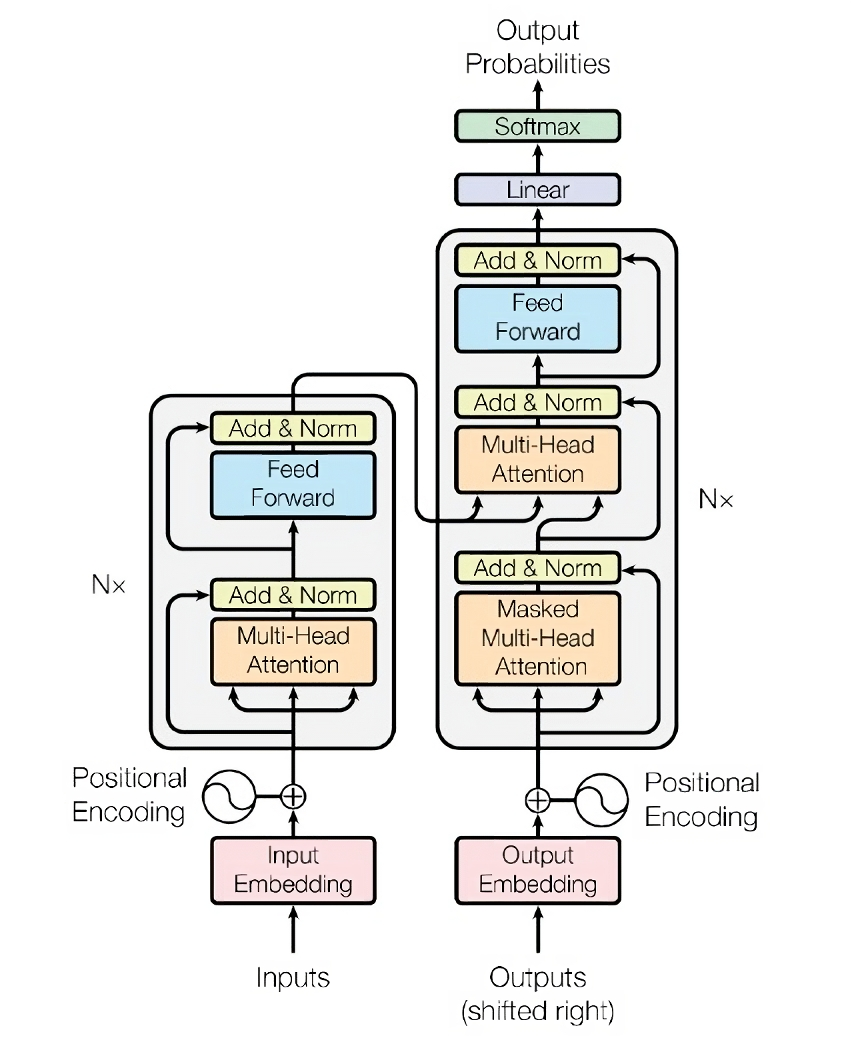
\includegraphics[width=9cm]{transformer}
    \caption{The Transformer - model architecture. from Ashish Vaswani et. al. [Attention is all you need]}
    \label{fig:galaxy}
\end{figure}



Bidirectional Encoder Representations from Transformers (BERT), introduced in 2018, stands as a remarkable milestone in the field of natural language processing (NLP). Its core innovation lies in its ability to pre-train comprehensive, bidirectional word understandings from unannotated text. Unlike its predecessors, BERT considers both left and right context in all its layers, rendering it exceptionally adaptable for a wide range of NLP tasks.
BERT's adaptability is one of its standout features, as it can be fine-tuned with minor adjustments for various tasks, such as question answering and language inference. These adjustments typically involve the addition of a single output layer, allowing BERT to consistently achieve top-tier results in diverse applications without the need for extensive task-specific architectural changes. BERT's pre-training process involves two primary tasks: the Masked Language Model (MLM), which entails predicting masked words based on surrounding context, and the Next Sentence Prediction (NSP), assessing if one sentence logically follows another in a document. Following pre-training, BERT can be tailored for specific downstream NLP tasks, ranging from text classification and named entity recognition to sentiment analysis. Various BERT models, including "BERT-Base" and "BERT-Large," have emerged to cater to different needs, cementing their pivotal role in a wide array of NLP applications.


To address challenges like overfitting, new techniques have been introduced, including Self-supervised Attention (SSA) and co-training frameworks, optimizing BERT's performance. SSA, in particular, contributes to enhancing the model's performance in auxiliary tasks by assigning task-specific weights to each word, reducing noise and improving overall performance.


However, the journey didn't stop at BERT, as it was found that the model was significantly undertrained. An improved recipe for training BERT models, known as RoBERTa, was proposed. RoBERTa builds upon the BERT model and fine-tunes its training methodology to achieve even better performance in various natural language understanding tasks. The modifications include a longer training duration with larger batches, an increase in the volume of training data, the removal of the next sentence prediction objective, broader scope by incorporating longer sequences in the training data, and dynamic changes to the masking pattern applied during training. These adjustments are meticulously designed to enhance the model's training efficiency and overall performance, marking yet another milestone in the ever-evolving landscape of NLP.

In 2018, the groundbreaking GPT-1 model, also known as GPT(Generative Pretrained Transformers), made its debut, primarily focusing on the training of a generative language model within the innovative Transformer framework using unsupervised learning. This approach aimed to overcome the challenges posed by the scarcity of labeled data by capitalizing on vast amounts of unlabeled and diverse examples. GPT-1, characterized as an auto-regressive decoder-only Transformer, incorporated the self-attention mechanism into its architecture. The model's training began with the BooksCorpus dataset, followed by fine-tuning for specific downstream tasks. Impressively, it demonstrated its versatility by surpassing state-of-the-art models in 9 out of 12 test datasets, spanning various Natural Language Processing (NLP) categories, hinting at a promising direction for advancing Artificial General Intelligence (AGI).

In 2019, GPT-2 emerged as a significant development, introducing multi-task learning while boasting a substantial increase in network parameters and training data compared to its predecessor. This enhancement allowed the model to exhibit a remarkable level of generalization across an array of supervised subtasks without requiring additional fine-tuning. With a tenfold increase in parameters and training on the extensive WebText corpus, GPT-2 achieved state-of-the-art performance levels in 7 out of 8 language modeling tasks, all within a zero-shot learning context. These results established baseline performances, stimulating further exploration for fine-tuning in specific applications.

GPT-3, released in 2020, took a significant leap with a staggering 175 billion parameters and a high-quality training dataset comprising around 500 billion tokens from major data repositories. GPT-3 introduced a novel approach by combining meta-learning and in-context learning, leading to substantial improvements in generalization capabilities. The model set a milestone as the first language model to exceed 100 billion parameters.

ChatGPT, a part of the GPT3.5 series models, demonstrated advanced capabilities in language comprehension and generation. It excelled in various language-related tasks, incorporating technologies like deep learning, unsupervised learning, instruction fine-tuning, multi-task learning, in-context learning, and reinforcement learning. The pilot version, InstructGPT, embraced reinforcement learning with human feedback (RLHF) to align better with user intent during interactions.

GPT-4, a powerful multimodal model, can process both image and text inputs, consistently outperforming humans on various exams. It leverages a Transformer-style architecture and undergoes pre-training on extensive datasets, including publicly available and third-party data. Fine-tuning is performed using Reinforcement Learning from Human Feedback (RLHF). What sets GPT-4 apart is its ability to handle prompts combining text and images, making it a versatile tool for vision and language tasks across various domains. In these scenarios, GPT-4 excels as it does with text-only inputs, marking a significant advancement in the field of AI.
 
\section{Proposed work}

\subsection{Extraction of Data}

The initial phase in the development of a conversational PDF chatbot involves text extraction from the PDF document. Multiple established technologies are available for this purpose, enabling the extraction of text from searchable PDFs. Notable options among these technologies include PyMuPDF, Pdfminer.six, and PyPdf2.

Based on the findings of a comparative analysis, each of these text extraction methods demonstrated a commendable level of accuracy within a relatively short timeframe. Notably, PyMuPDF outperformed the others, delivering the most precise results. Conversely, PyPdf2 yielded the output with the highest Levenshtein distance, tf-idf, and cosine similarity scores in comparison to the other two methods, making it a less favorable choice.

Both PyMuPDF and pdfminer.six exhibited similar tf-idf and cosine similarity scores, with PyMuPDF having a slightly higher Levenshtein distance than pdfminer.six. However, it's important to note that pdfminer.six required significantly more time to complete the extraction process when compared to PyMuPDF. Consequently, PyMuPDF emerges as the optimal choice for text extraction from PDF documents.

\begin{figure*}
    \centering
    \includegraphics[width=\textwidth]{flow}
    \caption{Proposed flowchart for P-BOT}
    \label{fig:your_image_label}
\end{figure*}

\subsection{Processing of Data}

The extraction of raw text from PDFs necessitates careful processing for effective storage and semantic search. An integral component of this process involves text chunking, a technique used to divide large text segments into smaller, more manageable units. Our examination highlights the impact of various chunking methods, including the NLTK Sentence Tokenizer, Spacy Sentence Splitter, and Langchain Character Text Splitter. Comparative analysis reveals that NLTK and Spacy consistently produce smaller, more digestible sentence segments, whereas Langchain generates larger and denser clusters of text.

Following the chunking process, the text segments are transformed into vector embeddings, numerical representations that capture word and sentence relationships. These embeddings are paramount for efficient storage and to improve semantic searches. By clustering related data points, they streamline the search process. Additionally, we investigate two distinct methods for generating these embeddings: OpenAI embeddings and Instructor embeddings. While OpenAI embeddings are known for their speed and accessibility via APIs, they come at a cost. In contrast, Instructor embeddings offer a budget-friendly alternative but exhibit slightly slower processing times.

\subsection{Storage of Data}

These embeddings are meticulously stored within specialized data repositories, commonly referred to as vector data stores. The vector data store is instrumental in streamlining the organization and retrieval of related data points, endowing LLMs with the capability to swiftly access and retrieve information. Several advanced technologies have emerged to facilitate the creation and utilization of vector data stores, including Facebook AI Similarity Search (FAISS), Pinecone, and Chroma. 

\subsection{Selection of Large language model}
We must choose a large language model capable of conducting query processing and semantic search within our vector datastore. To meet this requirement, we need a model that excels in natural language understanding, possesses context-awareness, and can generate pertinent responses or search results. Failure to satisfy these criteria could result in inaccurate, irrelevant, or misinterpreted query outcomes. Our research has identified several models that meet these requirements.

One of the most promising candidates is OpenAI's GPT-4, part of the GPT model family. It stands out as a versatile language model that can be fine-tuned for specific tasks, including query processing and semantic search. This adaptability makes it a valuable asset for applications such as search engines and chatbots. Another strong contender is RoBERTa, short for Robustly Optimized BERT Approach. As an enhanced iteration of the BERT model, RoBERTa excels in comprehending and generating human language text. Its bidirectional approach, considering both left and right context, enhances its capability to grasp the intricate relationships between words in queries and documents, making it a valuable resource for our task

\subsection{Query Processing}
Once a user query is accepted, it undergoes a series of processing steps before our expansive language model can generate a response. The objective is to transform the query into a format that closely resembles the data stored within our vector data store. Initially, the query is tokenized into smaller units, such as words or subwords, referred to as tokens. These tokens are more manageable and amenable to further processing. Subsequently, these tokens are transformed into vector embeddings, using the same method we used for  converting data from our PDF documents into embeddings.

Upon completing this transformation, the query is prepared for processing by the large language model. These models are built on the foundation of transformer architecture, which is exceptionally well-suited for handling sequential data, such as the query text. The transformer architecture is composed of numerous layers that incorporate self-attention and feedforward networks, enabling the model to capture intricate dependencies in the input text. The query, in its embedded form, progresses through the neural network in a forward pass, with each layer meticulously analyzing the query. This enables the model to grasp crucial context and establish relationships among tokens. The outcome is a precise interpretation of the query by the model, resulting in more accurate and context-aware responses.

\subsection{Searching and Generation of response}
At the core of this operation resides the vector database, where data undergoes a transformation into vector embeddings, encapsulating the latent semantic content. Each document or informational entity is densely linked with a vector representation, thereby facilitating expedient searches rooted in semantic similarity. The evaluation of this similarity can be determined using cosine similarity, a mathematical metric renowned for assessing the resemblance between two non-zero vectors within the expansive terrain of high-dimensional space.

Following this critical step, the large language model commences the semantic search phase, leveraging its comprehension of the user's query to systematically search the vector database for documents or information that are semantically related. Those distinguished by the most elevated similarity scores are accorded the status of utmost relevance.

After collecting these pertinent documents or informational insights, the language model proceeds to the final phase: the generation of responses. The generated response is contextually relevant to the user's query and can take various forms, depending on the application—ranging from concise answers to a list of pertinent documents or even detailed explanations.



\section{Prepare Your Paper Before Styling}

\subsection{Figures and Tables}
\paragraph{Positioning Figures and Tables} Place figures and tables at the top and 
bottom of columns. Avoid placing them in the middle of columns. Large 
figures and tables may span across both columns. Figure captions should be 
below the figures; table heads should appear above the tables. Insert 
figures and tables after they are cited in the text. Use the abbreviation 
``Fig.~\ref{fig}'', even at the beginning of a sentence.

\begin{table}[htbp]
\caption{Table Type Styles}
\begin{center}
\begin{tabular}{|c|c|c|c|}
\hline
\textbf{Table}&\multicolumn{3}{|c|}{\textbf{Table Column Head}} \\
\cline{2-4} 
\textbf{Head} & \textbf{\textit{Table column subhead}}& \textbf{\textit{Subhead}}& \textbf{\textit{Subhead}} \\
\hline
copy& More table copy$^{\mathrm{a}}$& &  \\
\hline
\multicolumn{4}{l}{$^{\mathrm{a}}$Sample of a Table footnote.}
\end{tabular}
\label{tab1}
\end{center}
\end{table}

\begin{figure}[htbp]
\caption{Example of a figure caption.}
\label{fig}
\end{figure}

Figure Labels: Use 8 point Times New Roman for Figure labels. Use words 
rather than symbols or abbreviations when writing Figure axis labels to 
avoid confusing the reader. As an example, write the quantity 
``Magnetization'', or ``Magnetization, M'', not just ``M''. If including 
units in the label, present them within parentheses. Do not label axes only 
with units. In the example, write ``Magnetization (A/m)'' or ``Magnetization 
\{A[m(1)]\}'', not just ``A/m''. Do not label axes with a ratio of 
quantities and units. For example, write ``Temperature (K)'', not 
``Temperature/K''.

\section*{Acknowledgment}

The preferred spelling of the word ``acknowledgment'' in America is without 
an ``e'' after the ``g''. Avoid the stilted expression ``one of us (R. B. 
G.) thanks $\ldots$''. Instead, try ``R. B. G. thanks$\ldots$''. Put sponsor 
acknowledgments in the unnumbered footnote on the first page.

\section*{References}


\begin{thebibliography}{00}
\bibitem{b1} J. Wu, W. Gan, Z. Chen, S. Wan, and H. Lin, "AI-generated content (AIGC): A survey," arXiv preprint arXiv:2304.06632, pp. 1–17, 2023.

\bibitem{b2} Wang, Y., Pan, Y., Yan, M., Su, Z., and Luan, T. H. (2023). "A Survey on ChatGPT: AI-Generated Contents, Challenges, and Solutions." arXiv preprint arXiv:2305.18339.

\bibitem{b3} Wu, T., He, S., Liu, J., Sun, S., Liu, K., Han, Q.L., and Tang, Y. (2023). "A brief overview of ChatGPT: The history, status quo, and potential future development." IEEE/CAA Journal of Automatica Sinica, 10(5), pp. 1122-1136.

\bibitem{b4} Gozalo-Brizuela, Roberto, and Eduardo C. Garrido-Merchan. "ChatGPT is not all you need. A State of the Art Review of large Generative AI models." arXiv preprint arXiv:2301.04655, 2023.

\bibitem{b5} L. Rabiner and B. Juang, "An introduction to hidden Markov models," in IEEE ASSP Magazine, vol. 3, no. 1, pp. 4-16, Jan 1986, doi: 10.1109/MASSP.1986.1165342.

\bibitem{b6} M. I. Mohd Yusoff, I. Mohamed and M. R. Abu Bakar, "Hidden Markov models: An insight," Proceedings of the 6th International Conference on Information Technology and Multimedia, Putrajaya, Malaysia, 2014, pp. 259-264, doi: 10.1109/ICIMU.2014.7066641.

\bibitem{b7} Viroli, C., and McLachlan, G. J. (2017). "Deep Gaussian mixture models." Statistics and Computing. doi:10.1007/s11222-017-9793-z.

\bibitem{b8} Pauls, Adam, and Dan Klein. "Faster and smaller n-gram language models." Proceedings of the 49th annual meeting of the Association for Computational Linguistics: Human Language Technologies. 2011.

\bibitem{b9} Niesler, Thomas R., and Philip C. Woodland. "A variable-length category-based n-gram language model." 1996 IEEE International Conference on Acoustics, Speech, and Signal Processing Conference Proceedings. Vol. 1. IEEE, 1996.

\bibitem{b10} Bickel, Steffen, Peter Haider, and Tobias Scheffer. "Predicting sentences using n-gram language models." Proceedings of human language technology conference and conference on empirical methods in natural language processing. 2005.

\bibitem{b11} Zong, Mingyu, and Bhaskar Krishnamachari. "A survey on GPT-3." arXiv preprint arXiv:2212.00857 (2022).

\bibitem{b12} Radford, Alec, Karthik Narasimhan, Tim Salimans, and Ilya Sutskever. "Improving language understanding by generative pre-training." (2018).

\bibitem{b13} Radford, A., Wu, J., Child, R., Luan, D., Amodei, D., and Sutskever, I. (2019). "Language models are unsupervised multitask learners." OpenAI blog, 1(8), p.9.

\bibitem{b14} Y. Zhang and Q. Yang, "A survey on multi-task learning," IEEE Trans. Knowl. Data Eng., vol. 34, no. 12, pp. 5586–5609, Dec. 2022.

\bibitem{b15} Y. Q. Wang, Q. M. Yao, J. T. Kwok, and L. M. Ni, "Generalizing from a few examples: A survey on few-shot learning," ACM Comput. Surv., vol. 53, no. 3, p. 63, May 2021.

\bibitem{b16} M. Khosla, A. Anand, and V. Setty, "A comprehensive comparison of unsupervised network representation learning methods," arXiv preprint arXiv:1903.07902, 2019.

\bibitem{b17} C. Ieracitano, A. Paviglianiti, M. Campolo, A. Hussain, E. Pasero, and F. C. Morabito, "A novel automatic classification system based on hybrid unsupervised and supervised machine learning for electrospun nanofibers," IEEE/CAA J. Autom. Sinica, vol. 8, no. 1, pp. 64–76, Jan. 2021.

\bibitem{b18} T. B. Brown, B. Mann, N. Ryder, M. Subbiah, J. Kaplan, P. Dhariwal, A. Neelakantan, P. Shyam, G. Sastry, A. Askell, S. Agarwal, A. Herbert-Voss, G. Krueger, T. Henighan, R. Child, A. Ramesh, D. M. Ziegler, J. Wu, C. Winter, C. Hesse, M. Chen, E. Sigler, M. Litwin, S. Gray, B. Chess, J. Clark, C. Berner, S. McCandlish, A. Radford, I. Sutskever, and D. Amodei, "Language models are few-shot learners," in Proc. 34th Int. Conf. Neural Information Processing Systems, Vancouver, Canada, 2020, pp. 1877–1901.

\bibitem{b19} Finn, C., Abbeel, P., and Levine, S. (2017). "Model-agnostic meta-learning for fast adaptation of deep networks." in Proc. 34th Int. Conf. Machine Learning, Sydney, Australia, 2017, pp. 1126–1135.

\bibitem{b20} Beck, J., Vuorio, R., Liu, E. Z., Xiong, Z., Zintgraf, L., Finn, C., and Whiteson, S. (2023). "A survey of meta-reinforcement learning." arXiv preprint arXiv:2301.08028.

\bibitem{b21} Dong, Q. X., Li, L., Dai, D. M., Zheng, C., Wu, Z. Y., Chang, B. B., Sun, X., Xu, J. J., Li, L., and Sui, Z. F. (2022). "A survey on in-context learning." arXiv preprint arXiv:2301.00234.

\bibitem{b22} Ouyang, L., Wu, J., Jiang, X., Almeida, D., Wainwright, C. L., Mishkin, P., Zhang, C., Agarwal, S., Slama, K., Ray, A., Schulman, J., Hilton, J., Kelton, F., Miller, L., Simens, M., Askell, A., Welinder, P., Christiano, J., Leike, J., and Lowe, R. (2022). "Training language models to follow instructions with human feedback." arXiv preprint arXiv:2203.02155.

\bibitem{b23} OpenAI, "Gpt-4 technical report," 2023. [Online]. Available: https://cdn.openai.com/papers/gpt-4.pdf.

\bibitem{b24} Jordan Hoffmann, Sebastian Borgeaud, Arthur Mensch, Elena Buchatskaya, Trevor Cai, Eliza Rutherford, Diego de Las Casas, Lisa Anne Hendricks, Johannes Welbl, Aidan Clark, et al. "Training compute-optimal large language models." arXiv preprint arXiv:2203.15556, 2022.

\bibitem{b25} Aakanksha Chowdhery, Sharan Narang, Jacob Devlin, Maarten Bosma, Gaurav Mishra, Adam Roberts, Paul Barham, Hyung Won Chung, Charles Sutton, Sebastian Gehrmann, et al. "PaLM: Scaling language modeling with pathways." arXiv preprint arXiv:2204.02311, 2022.

\bibitem{b26} Jack W Rae, Sebastian Borgeaud, Trevor Cai, Katie Millican, Jordan Hoffmann, Francis Song, John Aslanides, Sarah Henderson, Roman Ring, Susannah Young, et al. "Scaling language models: Methods, analysis and insights from training gopher." arXiv preprint arXiv:2112.11446, 2021.

\bibitem{b27} Jason Wei, Xuezhi Wang, Dale Schuurmans, Maarten Bosma, Ed Chi, Quoc Le, and Denny Zhou. "Chain-of-thought prompting elicits reasoning in large language models." NeurIPS, 2022.

\bibitem{b28} Jiaxin Huang, Shixiang Shane Gu, Le Hou, Yuexin Wu, Xuezhi Wang, Hongkun Yu, and Jiawei Han. "Large language models can self-improve." arXiv preprint arXiv:2210.11610, 2022.

\bibitem{b29} Z. Liang and S. Zhang. "Generating and Measuring Similar Sentences Using Long Short-Term Memory and Generative Adversarial Networks," in IEEE Access, vol. 9, pp. 112637-112654, 2021, doi: 10.1109/ACCESS.2021.3103669.

\bibitem{b30} Singh, Sushant, and Ausif Mahmood. "The NLP cookbook: modern recipes for transformer-based deep learning architectures." IEEE Access 9 (2021): 68675-68702.

\bibitem{b31} Jin, Kyohoon, et al. "Generative Data Augmentation via Wasserstein Autoencoder for Text Classification." 2022 13th International Conference on Information and Communication Technology Convergence (ICTC). IEEE, 2022.

\bibitem{b32} Chen, Yiren, et al. "Improving bert with self-supervised attention." IEEE Access 9 (2021): 144129-144139.

\bibitem{b33} Kowsher, Md, et al. "Bangla-BERT: transformer-based efficient model for transfer learning and language understanding." IEEE Access 10 (2022): 91855-91870.

\bibitem{b34} Vaswani, Ashish, et al. "Attention is all you need." Advances in neural information processing systems 30 (2017).

\bibitem{b35} Wolf, Thomas, et al. "Transformers: State-of-the-art natural language processing." Proceedings of the 2020 conference on empirical methods in natural language processing: system demonstrations. 2020.

\bibitem{b36} H. Palangi, L. Deng, Y. Shen, J. Gao, X. He, J. Chen, X. Song, and R. Ward, "Deep sentence embedding using long short-term memory networks: Analysis and application to information retrieval," IEEE/ACM Trans. Audio, Speech, Language Process., vol. 24, no. 4, pp. 694–707, Apr. 2016.

\bibitem{b37} S. Hochreiter and J. Schmidhuber, "Long short-term memory," Neural Comput., vol. 9, no. 8, pp. 1735–1780, 1997.

\bibitem{b38} A. Krizhevsky, I. Sutskever, and G. E. Hinton, "ImageNet classification with deep convolutional neural networks," Commun. ACM, vol. 60, no. 6, pp. 84–90, Jun. 2017.

\bibitem{b39} T. Mikolov, M. Karafiát, L. Burget, J. Černocký, and S. Khudanpur, "Recurrent neural network based language model," in Proc. 11th Annu. Conf. Int. Speech Commun. Assoc., Chiba, Japan, 2010, pp. 1045–1048.

\bibitem{b40} I. Sutskever, O. Vinyals, and Q. V. Le, "Sequence to sequence learning with neural networks," in Proc. Neural Inf. Process. Syst., Montreal, QC, Canada, 2014, pp. 3104–3112.

\bibitem{b41} S. R. Zhang, Z. Y. Liang, and J. Lin, "Sentence similarity measurement with convolutional neural networks using semantic and syntactic features," Comput., Mater. Continua, vol. 63, no. 2, pp. 943–957, 2020.

\bibitem{b42} X. Liu, P. He, W. Chen, and J. Gao, "Multi-task deep neural networks for natural language understanding," in Proc. 57th Annu. Meeting Assoc. Comput. Linguistics, Florence, Italy, 2019, pp

\bibitem{b43} J. Mueller and A. Thyagarajan, ‘‘Siamese recurrent architectures for learn-ing sentence similarity,’’ in Proc. 13th Conf. Artif. Intell., Phoenix, AZ, USA, 2016, pp. 2786–2792.

\bibitem{b44}I. J. Goodfellow, J. Pouget-Abadie, M. Mirza, B. Xu, D. Warde-Farley, S. Ozair, A. Courville, and Y. Bengio, ‘‘Generative adversarial nets,’’ain Proc. Neural Inf. Process. NIPS, Montreal, QC, Canada, 2014, pp. 2672–2680.

\bibitem{b45} J. Gui, Z. Sun, Y. Wen, D. Tao, and J. Ye, ‘‘A review on generative adversarial networks: Algorithms, theory, and applications,’’ Comput. Res. Repository, vol. abs/2001.06937, pp. 1–28, Jan. 2020.

\bibitem{b46} Z. Zhang, S. Liu, M. Li, M. Zhou, and E. Chen, ‘‘Bidirectional generative adversarial networks for neural machine translation,’’ in Proc. Assoc. Comput. Linguistics, Brussels, Belgium, no. 1, 2018, pp. 190–199.

\bibitem{b47} Y. Fu, Y. S. Feng, and J. P. Cunningham, ‘‘Paraphrase generation with latent bag of words,’’ in Proc. Neural Inf. Process. NIPS, Vancouver, BC, Canada, 2019, pp. 13623–13634.

\bibitem{b48}  C.-Y. Lin and E. Hovy, ‘‘Manual and automatic evaluation of summaries,’’ in Proc. Workshop Autom. Summarization (ACL), Barcelona, Spain, 2004, pp. 74–81.

\bibitem{b49} S. Bird, E. Klein, and E. Loper, Natural Language Processing With Python: Analyzing Text With the Natural Language Toolkit, vol. 44, 1st ed. Sebastopol, CA, USA: O’Reilly Media, 2009, pp. 421–424.

\bibitem{b50} C. Manning, M. Surdeanu, J. Bauer, J. Finkel, S. Bethard, and D. McClosky, ‘‘The Stanford CoreNLP natural language processing toolkit,’’ in Proc. 52nd Annu. Meeting Assoc. Comput. Linguistics, Syst. Demonstrations, Baltimore, MD, USA, 2014, pp. 55–60.

\bibitem{b51} J. Devlin, M.-W. Chang, K. Lee, and K. Toutanova, ‘‘BERT: Pre-training of deep bidirectional transformers for language understanding,’’ in Proc. Conf. North Amer. Chapter Assoc. Comput. Linguistics, Hum. Lang. Tech-nol., vol. 1, Jun. 2019, pp. 4171–4186.

\bibitem{b52} Y. Liu, M. Ott, N. Goyal, J. Du, M. Joshi, D. Chen, O. Levy, M. Lewis, L. Zettlemoyer, and V. Stoyanov, ‘‘RoBERTa: A robustly optimized BERT pretraining approach,’’ 2019, arXiv:1907.11692. [Online]. Available: http://arxiv.org/abs/1907.11692

\bibitem{b53} X. Wu, S. Lv, L. Zang, J. Han, and S. Hu, ‘‘Conditional bert contextual aug-mentation,’’ in Proc. Int. Conf. Comput. Sci. Cham, Switzerland: Springer,2019, pp. 84–95.

\bibitem{b54} Z. Yang, D. Yang, C. Dyer, X. He, A. Smola, and E. Hovy, ‘‘Hierarchical attention networks for document classification,’’ in Proc. Conf. North Amer. Chapter Assoc. Comput. Linguistics, Hum. Lang. Technol., 2016, pp. 1480–1489.

\bibitem{b55} Z. Lin, M. Feng, C. N. dos Santos, M. Yu, B. Xiang, B. Zhou, and Y. Bengio, ‘‘A structured self-attentive sentence embedding,’’ 2017, arXiv:1703.03130.

\bibitem{b56} A. Wang, A. Singh, J. Michael, F. Hill, O. Levy, and S. Bowman, ‘‘Glue: A multi-task benchmark and analysis platform for natural language under-standing,’’ in Proc. EMNLP Workshop BlackboxNLP, Analyzing Interpret-ing Neural Netw. (NLP), 2018, pp. 353–355.

\bibitem{b57} Hu, Dichao. ”An introductory survey on attention mechanisms in NLP problems.” Proceedings of SAI Intelligent Systems Conference. Springer, Cham, 2019.

\bibitem{b58} Luong, Minh-Thang, Hieu Pham, and Christopher D. Manning. ”Effective approaches to attention-based neural machine translation.” arXiv preprint arXiv:1508.04025 (2015).
\end{thebibliography}
\vspace{12pt}
\color{red}


\end{document}